\documentclass[10pt,letterpaper]{article}
\usepackage[top=0.85in,left=1.0in,footskip=0.75in]{geometry}

% amsmath and amssymb packages, useful for mathematical formulas and symbols
\usepackage{amsmath,amssymb}

% Use adjustwidth environment to exceed column width (see example table in text)
\usepackage{changepage}

% Use Unicode characters when possible
\usepackage[utf8x]{inputenc}

% textcomp package and marvosym package for additional characters
\usepackage{textcomp,marvosym}

% cite package, to clean up citations in the main text. Do not remove.
\usepackage{cite}

% Use nameref to cite supporting information files (see Supporting Information section for more info)
\usepackage{nameref,hyperref}

% line numbers
\usepackage[right]{lineno}

% ligatures disabled
\usepackage{microtype}
\DisableLigatures[f]{encoding = *, family = * }

% color can be used to apply background shading to table cells only
\usepackage[table]{xcolor}

% array package and thick rules for tables
\usepackage{array}

\usepackage{csquotes}

% create "+" rule type for thick vertical lines
\newcolumntype{+}{!{\vrule width 2pt}}

% create \thickcline for thick horizontal lines of variable length
\newlength\savedwidth
\newcommand\thickcline[1]{%
  \noalign{\global\savedwidth\arrayrulewidth\global\arrayrulewidth 2pt}%
  \cline{#1}%
  \noalign{\vskip\arrayrulewidth}%
  \noalign{\global\arrayrulewidth\savedwidth}%
}

% \thickhline command for thick horizontal lines that span the table
\newcommand\thickhline{\noalign{\global\savedwidth\arrayrulewidth\global\arrayrulewidth 2pt}%
\hline
\noalign{\global\arrayrulewidth\savedwidth}}


% Remove comment for double spacing
%\usepackage{setspace} 
%\doublespacing

% Text layout
\raggedright
\setlength{\parindent}{0.5cm}
\textwidth 6.5in 
\textheight 8.75in

% Bold the 'Figure #' in the caption and separate it from the title/caption with a period
% Captions will be left justified
\usepackage[aboveskip=1pt,labelfont=bf,labelsep=period,justification=raggedright,singlelinecheck=off]{caption}
\renewcommand{\figurename}{Fig}

% Use the PLoS provided BiBTeX style
\bibliographystyle{plos2015}

% Remove brackets from numbering in List of References
\makeatletter
\renewcommand{\@biblabel}[1]{\quad#1.}
\makeatother

% Leave date blank
\date{}

% Header and Footer with logo
\usepackage{lastpage,fancyhdr,graphicx}
\usepackage{epstopdf}
\pagestyle{myheadings}
\pagestyle{fancy}
\fancyhf{}
\setlength{\headheight}{27.023pt}
%\lhead{
\includegraphics[width=2.0in]{PLOS-submission.eps}}
\rfoot{\thepage/\pageref{LastPage}}
\renewcommand{\footrule}{\hrule height 2pt \vspace{2mm}}
\fancyheadoffset[L]{2.25in}
\fancyfootoffset[L]{2.25in}
%\lfoot{\sf PLOS}

%% Include all macros below

\newcommand{\lorem}{{\bf LOREM}}
\newcommand{\ipsum}{{\bf IPSUM}}

%% END MACROS SECTION


\begin{document}
\vspace*{0.2in}

% Title must be 250 characters or less.
\begin{flushleft}
{\Large
\textbf\newline{Microvessel Chaste: A Library for Multi-Scale Agent-Based Simulation of Tissues with Microvessels} % Please use "title case" (capitalize all terms in the title except conjunctions, prepositions, and articles).
}
\newline
% Insert author names, affiliations and corresponding author email (do not include titles, positions, or degrees).
\\
James A. Grogan\textsuperscript{1*},
Anthony J. Connor\textsuperscript{1, 2},
%B. Markelc\textsuperscript{3},
%R.J. Muschel\textsuperscript{3},
Philip K. Maini\textsuperscript{1},
Helen M. Byrne\textsuperscript{1},
Joe M. Pitt-Francis\textsuperscript{2}
\\
\bigskip
\textbf{1} Wolfson Centre for Mathematical Biology, Mathematical Institute, University of Oxford, Oxford, \mbox{OX2 6GG}, UK.
\\
\textbf{2} Department of Computer Science, University of Oxford, Oxford, \mbox{OX1 3QD}, UK.
\\
%\textbf{3} CRUK/MRC Oxford Institute for Radiation Oncology, University of Oxford, Oxford, \mbox{OX3 7DQ}, UK.
\bigskip

%\textcurrency Current Address: [JG Add current address for AJ].

* grogan@maths.ox.ac.uk

\end{flushleft}

\section*{Abstract}
Microvessel Chaste is an open-source software library for multi-scale agent-based modelling of tissues with microvessels. Development has focused on applications in spatial modelling of tumours and wound healing. Problems of interest in these areas include modelling blood flow, angiogenesis, and diffusible chemicals. This library integrates discrete representations of microvessels with re-usable components for agent-based modelling in the open-source Chaste library, such as discrete cells, meshes and ordinary and partial differential equation (ODE/PDE) solvers. The aims of the library are to facilitate i) rapid model composition from a range of interchangeable sub-models, ii) management of a large number of input parameters from various literature sources and iii) integration of modelling with experimental observations. These aims are pertinent in the area of discrete vascular tissue modelling, where model cross-comparison and experimental validation are still in their early stages. This article includes simple example applications of the library, which can be run on a desktop computer. The source code is available to download under an open-source Berkeley Software Distribution (BSD) licence at \url{https://jmsgrogan.github.io/MicrovesselChaste/}, together with details of a mailing list and links to documentation and tutorials.

\linenumbers

% Use "Eq" instead of "Equation" for equation citations.
\section*{Introduction}
Cancer, Heart And Soft Tissue Environment (Chaste)~\cite{Mirams2013} is an open-source C++ library for problems in computational physiology and biology. Chaste has been widely used to solve cardiac electrophysiology models~\cite{Cooper2015} and to develop multi-scale agent-based tissue models for developmental biology~\cite{Tetley2016} and cancer~\cite{Dunn2016}. Microvessel Chaste is an `add-on' project for Chaste, with functionality for including discrete microvessels in agent-based tissue models.

There are many dedicated software frameworks for agent-based cell modelling, including Chaste, CompuCell3D~\cite{Swat2012}, EPISIM~\cite{Sutterlin2013} and PhysiCell~\cite{Macklin2012}, however to the authors' knowledge, there is no similar framework for agent-based modelling of tissue with microvessels. Such computational models are widely used in tumour and wound healing~\cite{Owen2011}, vascular patterning (such as in development)~\cite{Secomb2013} and orthopaedic modelling~\cite{Carlier2012}. Multi-scale agent-based modelling of tissue with microvessels introduces several requirements in addition to those of cell modelling software. For example, i) centre-line or spatially resolved representations of vessels are needed in place of point or centre-based representations of cells, ii) blood flow and chemical transport problems are solved in vessel networks whose geometry and connectivity are constantly evolving and iii) new vessels may form and migrate based on mechanical and chemical cues. 

There are many notable bespoke computational models of tissue microvasculature, including Anderson and Chaplain~\cite{Anderson1998}, Alarcon \emph{et al.}~\cite{Alarcon2006}, Friboes \emph{et al.}~\cite{Frieboes2007}, Shirinifard \emph{et al.}~\cite{Shirinifard2009}, Owen \emph{et al.}~\cite{Owen2011}, Perfahl \emph{et al.}~\cite{Perfahl2011}, Welter and Rieger~\cite{Welter2013}, Secomb \emph{et al.}~\cite{Secomb2013}, and Boas and Merks~\cite{Boas2015}, aimed at answering specific questions. Our aim is to develop general software with the following attributes: i) availability under a permissive open-source license, ii) API documentation and user tutorials, iii) capability for on- and off-lattice modelling of vessels in arbitrary geometries in two and three dimensions and iv) use of object-oriented programming for \emph{extensibility}. In addition, the software is based on C++ for computational \emph{efficiency} and Boost Units~\cite{boost161} for compile-time dimensional analysis, input parameter management and improved \emph{reliability}. 

The aforementioned attributes allow future utilization of the library in addressing two outstanding challenges in tissue microvasculature modelling. \emph{First}, the importance of rapidly constructing and cross-comparing multi-scale agent-based models of tissue microvasculature is well recognized, as are the challenges in developing software for such an endeavour~\cite{Rieger2015, Connor2012}. Due to the lack of open-source, documented software, it is currently necessary to re-implement each computational model before application, delaying comparison studies and reducing reproducibility. \emph{Second}, there is now a wealth of high resolution three-dimensional (3D) experimental imaging data against which model predictions can be compared~\cite{Tozer2004}. To fully exploit these data it is necessary that 3D tissue regions of reasonable volume with realistic geometries can be simulated, as per Grogan \emph{et al.}~\cite{Grogan2016}. There are few approaches developed for this purpose in the literature. This functionality is available in the Microvessel Chaste library, including previously unpublished methods for 3D off-lattice modelling of sprouting angiogenesis.  

While the authors have previously developed and applied a range of multi-scale agent-based microvessel models in the areas of cancer~\cite{Alarcon2006, Perfahl2011, Grogan2016} and angiogenesis~\cite{Connor2015}, their incorporation in Microvessel Chaste is the first time such models have been made available open-source, with documentation and tutorials. Code design and implementation are discussed in the next section, followed by two sample applications. 	

\section*{Design and Implementation}

This section briefly summarizes available algorithms by demonstrating how the library can be used to construct and solve a typical multi-scale agent-based microvessel problem. Dedicated articles, such as Mirams~\emph{et al.}~\cite{Mirams2013}, should be consulted for further details on algorithms related to core Chaste functionality, including discrete cell modelling. At present, the library can be used with Linux only, with virtual machines required for use on Microsoft Windows and Mac OS X. To install Microvessel Chaste it is necessary to build from source after downloading and setting up dependencies. 

\subsection*{Algorithm Overivew}

The library is designed for composing multi-scale agent-based tissue problems with microvessels using on- and off-lattice representations of cells and vessels. While the library attempts to minimize the imposition of a definitive model structure on the user, it is helpful when introducing algorithms to consider a concrete use case. 

Fig~\ref{fig1} shows how the library can be used to \emph{compose} a problem of interest in tumour modelling. For further details on models of this type the reader is referred to Owen \emph{et al.}~\cite{Owen2011}. Here, an initial vessel network and cell population are constructed, transport partial differential equations (PDEs) for diffusible chemicals configured, and rules for vessel growth or shrinkage due to blood flow defined, along with rules for vessel sprouting and endothelial tip cell migration in a stimulus field. The ability to compose a model from a collection of sub-models is noted. There is a high degree of interaction between components. Once a domain, which is a geometrical feature in two dimensions (2D) or 3D, is defined it can be used in the construction of vessel networks and cell populations through multiple space-filling or boolean operations, and in the generation of a computational grid (mesh) for use in the solution of PDEs. Sub-models can be collected in hierarchical structures, for example a \textit{StructuralAdaptationSolver} can manage a \textit{FlowSolver} and is itself managed by a \textit{MicrovesselSolver}. Alternatively, sub-models can be executed in isolation, for example to simply solve a nutrient PDE with cell location dependent sink terms.

\begin{figure}[!h]
\centering
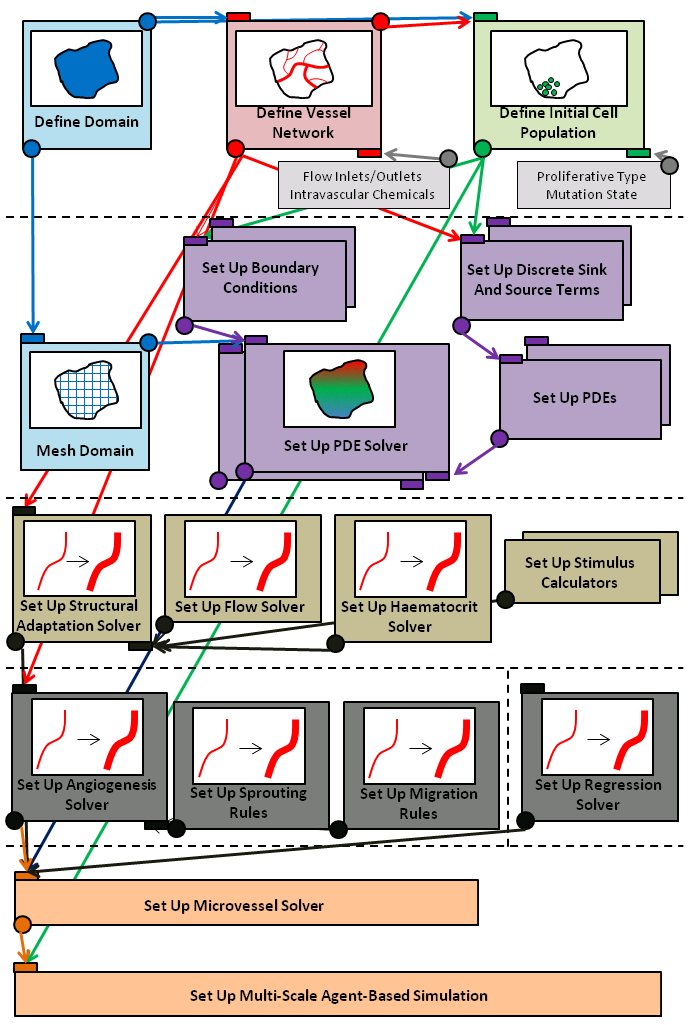
\includegraphics[width=0.7\textwidth]{Fig1.png}
\caption{{\bf An example of how a microvessel model can be composed using Microvessel Chaste.}
A schematic showing the composition of a tumour growth model using Microvessel Chaste. The ability to compose a model from a collection of sub-models is shown.}
\label{fig1}
\end{figure}

Fig~\ref{fig2} shows how the library can be used to \emph{solve} a problem of interest in tumour modelling. The user can decide on ordering themselves by suitably over-riding \textit{Solve()} and \textit{Increment()} methods. The steps on the left-hand side of Fig~\ref{fig2} are already implemented as part of the agent-based cell modelling in Chaste~\cite{Mirams2013}. The Microvessel Chaste library interacts with the cell-based solver as a plug-in (called a \textit{SimulationModifier} in Chaste), by modifying the contents of a cell population once per time step. In the example problem shown in Fig~\ref{fig2}, vessels interact with (non-vessel) cells only via their shared influence on the solutions of chemical transport problems. Cell birth, death and cell-cycle progression can be affected by the PDE solution, which is sampled by each cell during the \textit{CellDataUpdate()} step. More detailed interactions, such as cell-vessel spatial occlusion, or forming vessels from collections of discrete cells, are also possible.

\begin{figure}[!h]
\centering
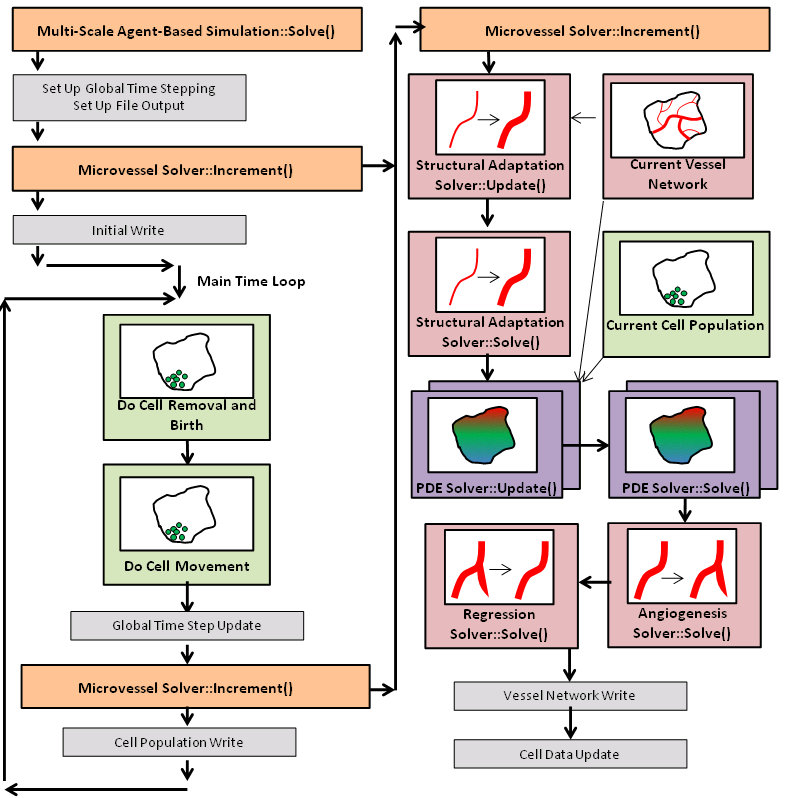
\includegraphics[width=0.8\textwidth]{Fig2.png}
\caption{{\bf An example of how a microvessel model can be solved using Microvessel Chaste.}
A schematic showing the solution of a tumour growth model using Microvessel Chaste. Cells can be marked for removal, division or movement by the \textit{MicrovesselSolver} ahead of the next global time step.}
\label{fig2}
\end{figure}

\subsection*{Code Layout And Design}

The components of the library are as follows:

\begin{itemize}
	\item geometry -- code for generating and describing 2D and 3D geometries using piecewise linear complex (PLC) descriptions for direct use in Tetgen~\cite{Si2015} meshing software,
	\item mesh -- code for automated finite element meshing of 2D and 3D geometries and interpolation of vessel and cell locations onto meshes and regular grids,
	\item ode -- ordinary differential equation (ODE) models for cell-cycling,
	\item pde -- descriptions and solvers for steady state linear and non-linear PDEs with discrete sinks and sources for vessels and cells. Solvers use finite differences, finite element methods and Green's function methods~\cite{Secomb2013} based on Boost uBLAS and PETSc for vector and matrix operations,
	\item population -- code for describing, reading, writing and generating vessel networks,
	\item simulation -- flow, structural adaptation and angiogenesis solvers. Simulation modifiers for integration of discrete vessel simulations with discrete cell simulations in Chaste,
	\item utility -- dimensional analysis and a collection of literature parameters of interest for tissue microvasculature simulations.	
\end{itemize}

Object-oriented programming, including templating in C++, are utilized throughout the library. Input and output of vessel networks, grids and PDE results are in VTK (Paraview) format, which allows the use of standard tools for visualization and post-processing. Python bindings are generated automatically using Py++ with a CASTXML back-end. Pre-compiled C++ classes can be overloaded in Python, without the need to re-compile the full framework. This overloading allows for automated, dynamic model (or sub-model) generation, for example using a mark-up language based input file. Given the variety of modelling paradigms and large number of input parameters used in problems of interest, there is much potential for misuse of units. Microvessel Chaste uses low-cost compile-time unit checking to ensure dimensional consistency and automatic solver-specific non-dimensionalisation through the Boost Units framework. The latter is useful for minimising floating pointer errors during the solution of PDEs and flow problems.

\section*{Results}

In this section two sample multi-scale agent-based problems are demonstrated, and are available for reproduction following wiki-based tutorials at \url{https://jmsgrogan.github.io/MicrovesselChaste/}.

\subsection*{A 2D Lattice-Based Tumour Simulation}

The first example is a 2D lattice-based tumour growth simulation following from Owen \emph{et al.}~\cite{Owen2011}, but with some simplifications to reduce computational expense. This example demonstrates the feasibility of replicating a well known tumour growth simulation, which is similar to many models in the literature~\cite{Anderson1998, Frieboes2007, Perfahl2011, Connor2015}. It also demonstrates how the library interfaces with the functionality of the Chaste discrete cell modelling software. Recent advances in intravital imaging allow in vivo observation of this process at the scale of individual cells, as shown in Fig~\ref{fig3}(a)\cite{Grogan2016}. These new techniques, which allow observation of biological processes at the same size-scale as the computational models, can be used for model initialization in Microvessel Chaste (as per Grogan et al.~\cite{Grogan2016}), and in the longer term, model validation.

% Place figure captions after the first paragraph in which they are cited.
\begin{figure}[!h]
\centering
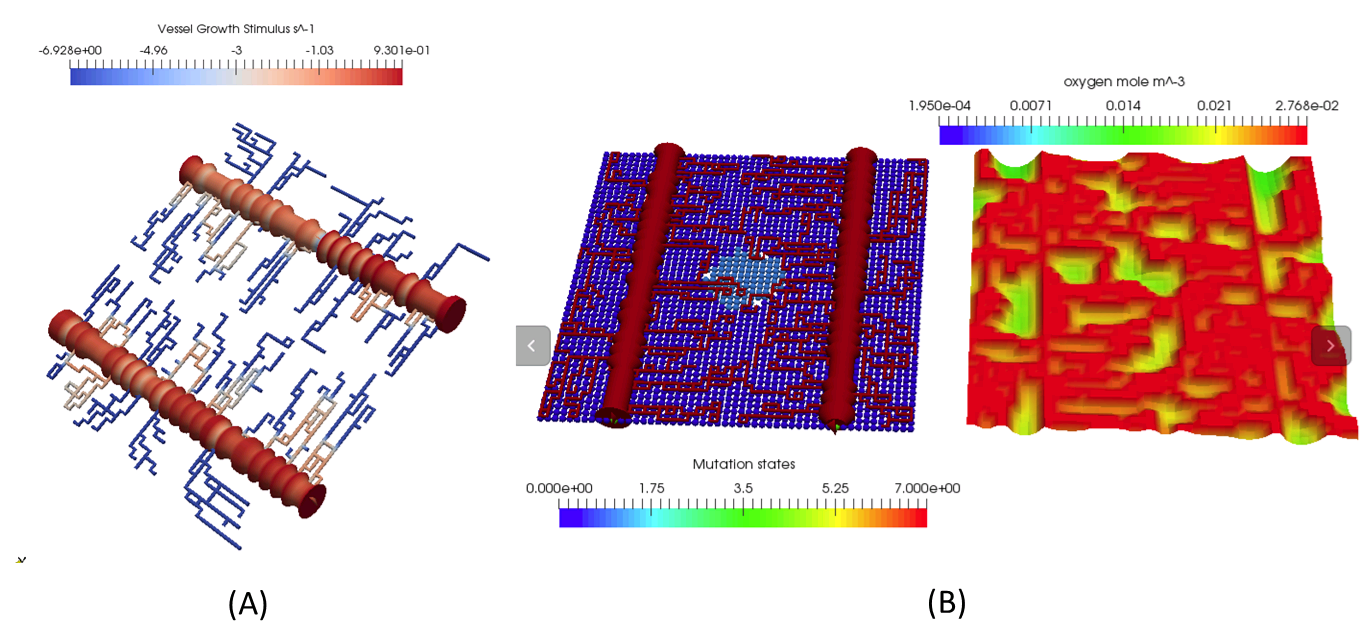
\includegraphics[width=0.8\textwidth]{Fig3.png}
\caption{{\bf A 2D lattice-based tumour simulation performed using the Microvessel Chaste library.}
(a) An experimental image of a tumour microvessel network (red) following administration of a Hoescht stain (blue), which stains DNA in tumour cells~\cite{Grogan2016}. This demonstrates the ability to image biological features at the same size-scale as the computational models. (b) A computational model of tumour growth over a period of 16 days using the Microvessel Chaste library. A planned application of the library is studying vascular patterning for comparison with observations from imaging data.}
\label{fig3}
\end{figure}

As shown in Fig~\ref{fig3}(b), the problem is initialized with two large, parallel, counter-flowing vessels, positioned on a regular lattice. A cellular automaton based cell population is used to fill all lattice sites, including those occupied by vessels. `Tumour' cell types are assigned to a central circular region and `Normal' types to the remainder. Due to their distance from the large vessels, cells will become hypoxic and release Vascular Endothelial Growth Factor (VEGF). This stimulates the sprouting and migration of new vessels toward the tumour. Eventually, cells far from the vessels become apoptotic, leaving only cores of viable cells encircling oxygenated vessels. The surviving tumour cells gradually invade the regions surrounding vessels at the expense of the normal cells. The process is similar to that observed in the simulations of Perfahl \emph{et al.}~\cite{Perfahl2011}.

There are many potential additions to models of this type which have been explored in the literature, including simulated administration of chemo-therapeutic and anti-angiogenic drugs~\cite{Alarcon2006} and radiotherapy~\cite{Grogan2016}, and the use of 3D domains~\cite{Perfahl2011}. All of these cases can be simulated using the Microvessel Chaste library.

\subsection*{A 3D Off-Lattice Angiogenesis Simulation}

The second example is a 3D off-lattice simulation of angiogenesis on a curved surface (see Fig~\ref{fig4}). This example demonstrates some of the advanced features of the library. These include geometry manipulation, 3D off-lattice angiogenesis and the solution of PDEs on 3D domains. The application is appropriate for the corneal micropocket assay that is widely used to study angiogenesis~\cite{Connor2015}. Typical experimental results are shown in \ref{fig4}(a). 

% Place figure captions after the first paragraph in which they are cited.
\begin{figure}[!h]
\centering
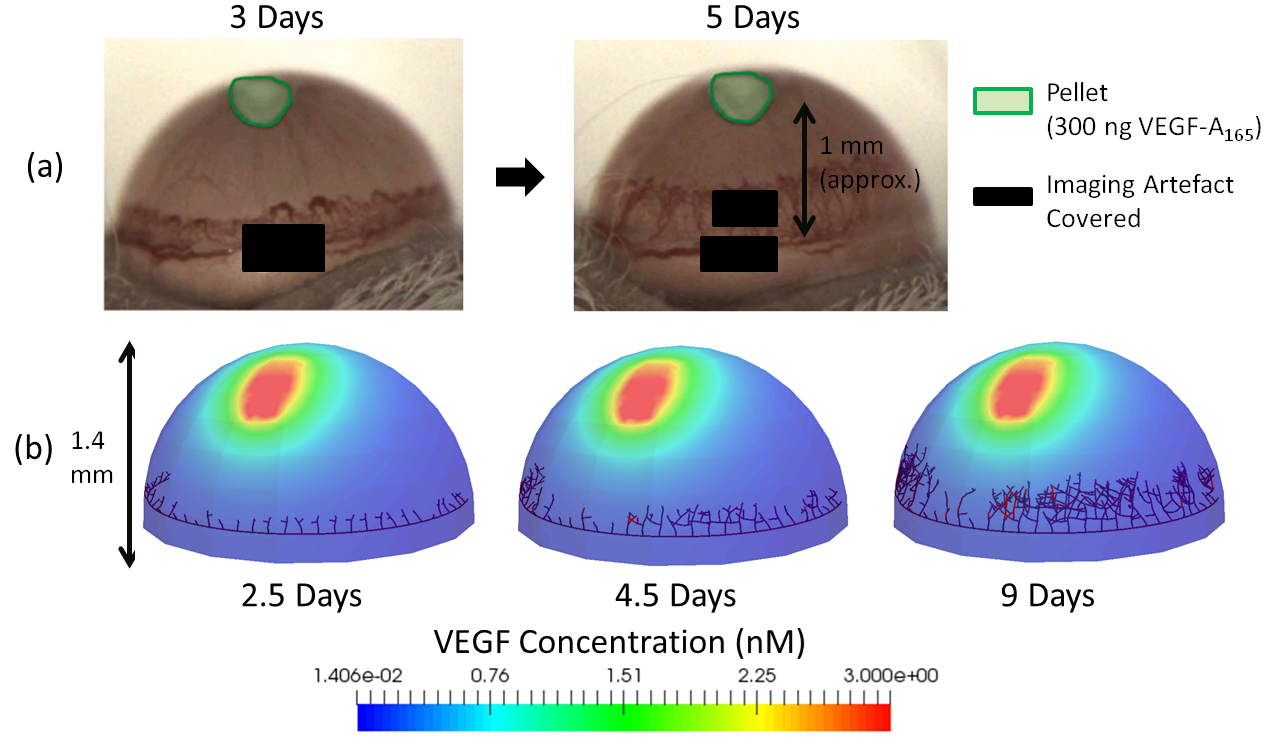
\includegraphics[width=0.8\textwidth]{Fig4.png}
\caption{{\bf A 3D off-lattice angiogenesis simulation performed using the Microvessel Chaste library.}
(a) Images from a cornea micropocket experiment showing microvessels (dark red) at 3-5 days post pellet implantation~\cite{Connor2015}. (b) Application of the Microvessel Chaste library in modelling a similar experiment, but with a number of simplifications for the purposes of the tutorial. The reader is referred to Connor \emph{et al.}~\cite{Connor2015} for a more detailed model.}
\label{fig4}
\end{figure}

In this assay a pellet containing an angiogenic growth factor (for example, VEGF) is implanted in the cornea. VEGF diffuses from the pellet into the corneal tissue and stimulates endothelial cells lining limbal vessels to form sprouts and migrate toward the pellet along VEGF gradients. This example follows a common modelling paradigm in which cells are treated as a continuum, but vessels are modelled as discrete agents~\cite{Secomb2013}. This reduces computational expense for the purposes of generating a tutorial. As shown in Fig~\ref{fig4}(b), the cornea is represented as a hemispherical domain of radius 1.4 mm and thickness 0.1 mm. The pellet is a cuboid with side length 0.3 mm and depth 0.1mm, with a prescribed VEGF concentration of 3.0 nM on the boundaries. In practice, the VEGF in the pellet will deplete. Vessels sprout from the limbal vessel and then follow a persistent random walk with bias towards other vessel tips and up VEGF gradients. The VEGF distribution is obtained by solving a diffusion PDE on the cornea at the start of the simulation. Vessels migrate toward the pellet, remaining within the volume of the 3D cornea geometry.

Possible extensions to this simple model could include the addition of discrete stromal cells, distinction between perfused and unperfused vessels and the use of multiple vessel growth factors, as per the model in Connor~\emph{et al.}~\cite{Connor2015}.

\section*{Availability and Future Directions}

Additional functionality for semi-automated 2D and 3D image segmentation and meshing is under development, to aid integration with experimental studies such as those shown in Fig~\ref{fig3}(a). Porting to Windows and Mac OS X are of interest. At present, algorithms operate in serial only, however there is scope for distributed memory parallelisation. All PDE and flow solvers are based on PETSc~\cite{Balay2014} structures and vessel network components may be communicated using existing serialization functionality in Chaste~\cite{Harvey2015} or through serialization of VTK objects~\cite{Schroeder2003}. As discussed in Mirams et al.~\cite{Mirams2013}, contributions are welcome via the main Chaste website, which includes a developer wiki, mailing list details and the ability to open and comment on work tickets. 

\section*{Acknowledgments}
The research leading to these results has received funding from the European Union's Seventh Framework Programme for research, technological development and demonstration under grant agreement No 600841. The authors acknowledge helpful inputs from the Chaste development team, in particular Jonathan Cooper, Alex Fletcher, James Osborne, Gary Mirams and Martin Robinson. We thank Bostjan Markelc and Ruth Muschel of the CRUK/MRC Oxford Institute for Radiation Oncology for providing the multi-photon image presented in Fig~\ref{fig3} and for useful discussions.

\nolinenumbers

\begin{thebibliography}{10}
%1
\bibitem{Mirams2013}
Mirams GR, Arthurs CJ, Bernabeu MO, Bordas R, Cooper J, Corrias A, Davit Y, Dunn S, Fletcher AG, Harvey DG, Marsh ME, Osborne JM, Pathmanathan P, Pitt-Francis J, Southern J, Zemzemi N, Gavaghan DJ.
\newblock {{C}haste: an open source C++ library for computational physiology and biology}.
\newblock PLoS Comp Bio. 2013 Jan;9(3):e1002970.

%2
\bibitem{Cooper2015}
Cooper J, Spiteri RJ, Mirams GR.
\newblock {{C}ellular cardiac electrophysiology modeling with Chaste and CellML}.
\newblock Front Physiol. 2015 Jan;5:511.

%3
\bibitem{Tetley2016}
Tetley RJ, Blanchard GB, Fletcher AG, Adams RJ, Sanson B.
\newblock {{U}nipolar distributions of junctional Myosin II identify cell stripe boundaries that drive cell intercalation throughout Drosophila axis extension}.
\newblock eLife. 2016 May;5:e12094.

%4
\bibitem{Dunn2016}
Dunn SJ, Osborne JM, Appleton PL, Nathke I.
\newblock {{C}ombined changes in Wnt signaling response and contact inhibition induce altered proliferation in radiation-treated intestinal crypts}.
\newblock Mol Biol Cell. 2016 June;27(11):1863-1874.

%5
\bibitem{Swat2012}
Swat M, Thomas GL, Belmonte JM, Shirinifard A, Hmeljak D, Glazier JA.
\newblock {{M}ulti-scale modeling of tissues using CompuCell3D}.
\newblock Method in Cell Biol. 2012;110:325-366.

%6
\bibitem{Sutterlin2013}
Sutterlin T, Kolb C, Dickhaus H, Jager D, Grabe N.
\newblock {{B}ridging the scales: semantic integration of quantitative SBML in graphical multi-cellular models and simulations with EPISIM and COPASI}.
\newblock Bioinformations. 2013 January;15(29):223-229.

%7
\bibitem{Macklin2012}
Macklin P, Edgerton ME, Thompson AM, Cristini V.
\newblock {{P}atient-calibrated agent-based modelling of ductal carcinoma in situ (DCIS): From microscopic measurements to macroscopic predictions of clinical progression}.
\newblock J Theor Biol. 2012;301:122-140.

%8
\bibitem{Owen2011}
Owen MR, Stamper J, Muthana M, Richardshon GW, Dobson J, Lewis CE, Byrne HM.
\newblock {{M}athematical modeling predicts synergistic antitumor effects of combining a macrophage-based, hypoxia-targeted gene therapy with chemotherapy}.
\newblock Cancer Res. 2015 April;71(8):2826-2837.

%9
\bibitem{Secomb2013}
Secomb TW, Alberding JP, Hsu R, DeWhirst MW, Pries AR.
\newblock {{A}ngiogenesis: an adaptive dynamic biological patterning problem}.
\newblock PLoS Comp Bio. 2013;9(3):e1002983.

%10
\bibitem{Carlier2012}
Carlier A, Geris L, Bentley K, Carmeliet G, Carmeliet P, Van Oosterwyck H.
\newblock {{M}OSAIC: A multiscale model of osteogenesis and sprouting angiogenesis with lateral inhibition of endothelial cells}.
\newblock PLoS Comp Bio. 2012;8(10):e1002724.

\bibitem{Anderson1998}
Anderson ARA, Chaplain MAJ.
\newblock {{C}ontinuous and discrete mathematical models of tumor-induced angiogenesis}.
\newblock Bullet Math Bio. 1998;60:857-900.

\bibitem{Frieboes2007}
Frieboes HB, Lowengrub JS, Wise S, Zheng X, Macklin P, Bearer E, Cristini V.
\newblock {{C}omputer simulation of glioma growth and morphology}.
\newblock Neuroimage. 2007;37(Supl 1):S59-S70.

\bibitem{Shirinifard2009}
Shirinifard A, Scott Gens J, Zaitlen L, Poplawski J, Swat M, Glazier JA.
\newblock {{3}D multi-cell simulation of tumor growth and angiogenesis}.
\newblock PLoS One. 2009;4(10):e7190.

\bibitem{Welter2013}
Welter M, Rieger H.
\newblock {{I}nterstitial fluid flow and drug delivery in vascularized tumors: a computational model}.
\newblock PLoS One. 2013;8(8):e70395.

\bibitem{Boas2015}
Boas SEM, Merks RMH.
\newblock {{T}ip cell overtaking occurs as a side effect of sprouting in computational models of angiogenesis}.
\newblock BMC Systems Bio. 2015;9(86):DOI 10.1186/s12918-015-0230-7.

\bibitem{boost161}
Boost Development Team.
\newblock {{B}oost Units Reference Guide}.
\newblock Available: \url{http://www.boost.org/doc/libs/1_61_0/doc/html/boost_units.html}.

\bibitem{Rieger2015}
Rieger H, Welter M.
\newblock {{I}ntegrative models of vascular remodeling during tumor growth}.
\newblock WIREs Syst Biol Med. 2015;7:113-129.

\bibitem{Connor2012}
Connor AJ, Cooper J, Byrne HM, Maini PK, McKeever S.
\newblock {{O}bject-oriented paradigms for modelling vascular tumor growth: a case study}.
\newblock In: The Fourth International Conference on Advances in Systems Simulation. Simul 2012. Iaria, Lisbon,74-83.

\bibitem{Tozer2004}
Tozer GM, Ameer-Berg SM, Baker J, Barber P, Hill SA, Hodgkiss R, Locke R, Prise V, Wilson I, Vojnovic B.
\newblock {{I}ntravital imaging of tumour vascular networks using multi-photon fluorescence microscopy}.
\newblock Advanced Drug Deliv Rev. 2005;57:135-152.

\bibitem{Grogan2016}
Grogan JA, Markelc B, Connor AJ, Muschel R, Pitt-Francis JM, Maini PK, Byrne HM.
\newblock {{P}redicting the influence of microvascular structure on tumour response to radiotherapy}.
\newblock IEEE Trans Biomed Eng 2016;In Press,DOI:10.1109/TBME.2016.2606563.

\bibitem{Alarcon2006}
Alarcon T, Owen MR, Byrne HM, Maini PK.
\newblock {{M} ultiscale modelling of tumour growth and therapy: the influence of vessel normalisation on chemotherapy}.
\newblock Computat and Math Method in Med. 2006;7(2-3):85-119.

\bibitem{Perfahl2011}
Perfahl H, Byrne HM, Chen T, Estrella V, Alarcon T, Lapin A, Gatenby R, Gillies RJ, Llord MC, Maini PK, Reuss M, Owen MR.
\newblock {{M}ultiscale modelling of vascular tumour growth in 3D: the roles of domain size and boundary conditions}.
\newblock PLoS One. 2011 April;6(4):e14790.

\bibitem{Connor2015}
Connor AJ, Radoslaw P, Nowak EL, Thomas M, Hertig F, Hoert S, Quaiser T, Schocat E, Pitt-Francis J, Cooper J, Maini PK, Byrne HM.
\newblock {{A}n integrated approach to quantitative modelling in angiogenesis research}.
\newblock J R Soc Interface. 2015 August;12:e20150546.

\bibitem{Si2015}
Si H.
\newblock {{T}etGen, a delaunay-based quality tetrahedral mesh generator}.
\newblock ACM Trans. on Mathematical Software. 2015;41(2):DOI:10.1145/2629697.

\bibitem{Harvey2015}
Harvey DG, Fletcher AG, Osborne JM, Pitt-Francis JM.
\newblock {{A} parallel implementation of an off-lattice individual-based model of multicellular populations}.
\newblock Comput Phys Comm. 2015;192:130-137.

\bibitem{Balay2014}
Balay S et al..
\newblock {{P}ETSc users manual revision 3.5}.
\newblock Technical Report, Argonne National Laboratory (ANL). June 2014.

\bibitem{Schroeder2003}
Schroeder W et al..
\newblock {{T}he Visualization Toolkit, 3rd Edition}.
\newblock  Kitware Inc.. 2003.

\end{thebibliography}


\end{document}

